\documentclass{article}
\usepackage{framed}
\usepackage{scrextend}
\usepackage{xcolor}
\usepackage[spanish,es-tabla]{babel}
\usepackage[dvips,a3paper,centering,margin=2cm]{geometry}
\usepackage{multicol}
\usepackage{subcaption}
\usepackage[utf8]{inputenc}
\usepackage{color}
\usepackage{float}
\usepackage{cite}
\usepackage{colortbl}
\usepackage{tabulary}
\usepackage{multirow}
\usepackage{amsmath}
\usepackage{graphicx}
\usepackage[breaklinks=true,hidelinks]{hyperref}
\definecolor{shadecolor}{RGB}{26, 147, 111}
\definecolor{rb}{rgb}{0.025,0.5,0.9} 
\definecolor{na}{rgb}{0.8274,0.305,0.196} 
\definecolor{title}{RGB}{26, 147, 111}
\definecolor{ver}{RGB}{255,255,255}
\pagestyle{empty}
\def\to{\rightarrow}
\begin{document}
\vspace*{-2cm}
\changefontsizes{14pt}
\hspace*{-1cm}
\begin{minipage}{0.2\linewidth}
\vspace{0.7cm}
\vspace*{-0.15cm}
\includegraphics[scale=0.12]{images/ifir.eps}
\end{minipage}
\vspace*{-0.4cm}
\begin{minipage}{0.6\linewidth}
\vspace*{0.7cm}
\begin{center}
\changefontsizes{15pt}
\hspace*{-0.1cm}
\textbf{\textcolor{title}{Análisis del PM\textsubscript{10} medido y el AOD\textsubscript{550nm} estimado a partir de las mediciones de irradiancia solar VIS-NIR en el Área Metropolitana de Monterrey}}
\end{center}
\vspace{-1cm}
\begin{center}
\changefontsizes{11pt}
Gamaliel López-Padilla$^1$, Adriana Ipiña$^{2}$, Constanza Zuñiga Villareal$^{1}$,Rubén Piacentini$^{2}$\\
1. Facultad de Ciencias Físico-Matemáticas,UANL, México\\
2. Instituto de Física Rosario,CONICET-UNR, Argentina\\
email: giovannilopez9808@gmail.com y ipina@ifir-conicet.gov.ar
\end{center}
\end{minipage}
\begin{minipage}{0.2\linewidth}
\hspace*{0.2cm}

\includegraphics[scale=0.2]{images/fcfm.eps}
\end{minipage}
\vspace{0.2cm}
\changefontsizes{12pt}
\begin{center}
\begin{shaded}
\textbf{\textcolor{ver}{Introducción}}
\end{shaded}
\end{center}
\begin{minipage}{0.47\linewidth}
\begin{figure}[H]
\centering
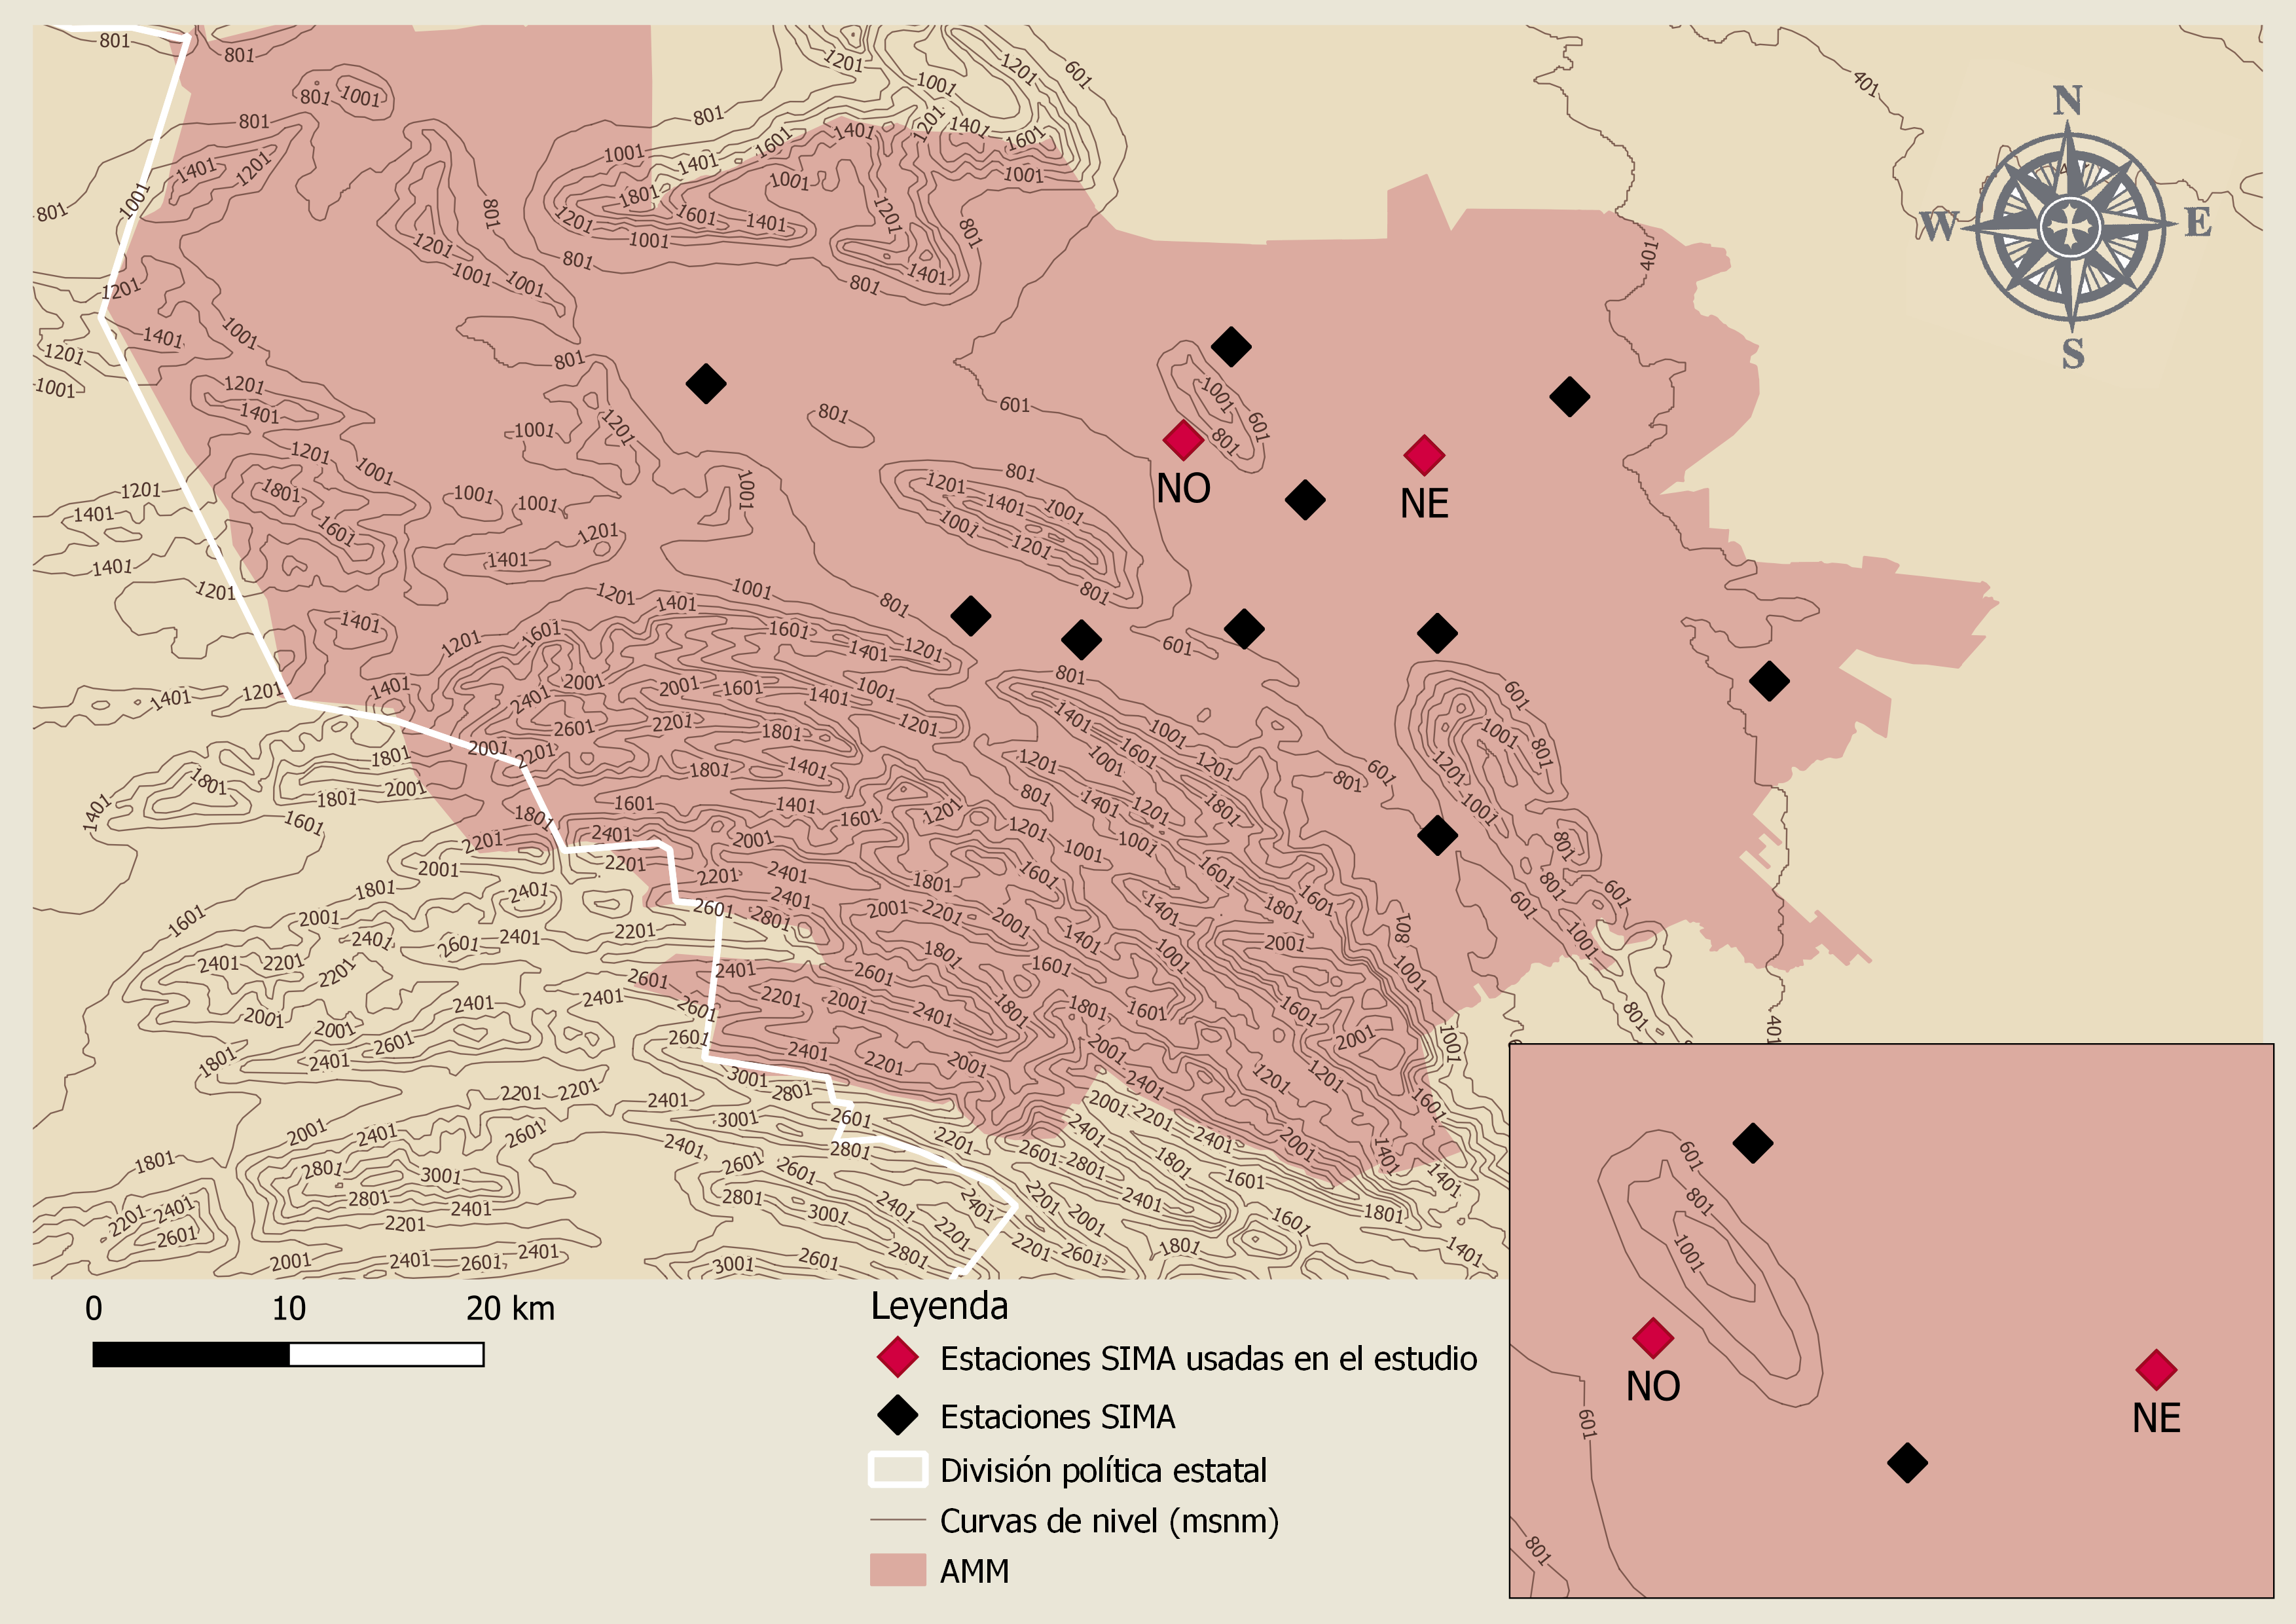
\includegraphics[scale=0.375]{images/AMM10.png}
\caption{Área Metropolitana de Monterrey (AMM)}
\end{figure}
\end{minipage}
\begin{center}
\begin{shaded}
\textbf{\textcolor{ver}{Metodologia}}
\end{shaded}
\end{center}
\begin{table}[H]
    \centering
    \begin{tabular}{ccccccccccc} 
         Escenario & CH\textsubscript{2}O & CH\textsubscript{4}& CO & HNO\textsubscript{2} & HNO\textsubscript{3} & NO & NO\textsubscript{2} & NO\textsubscript{3} & O\textsubscript{3} & SO\textsubscript{2}\\ \hline
       Pristine &-0.003 & 0  &-0.1  &-9.9x10$^{4}$& 0  &      0&    0  &    -4.9x10$^{-4}$  & OMI & 0 \\ \cline{1-9} \cline{11-11}
       Moderate & 0.007 & 0.3& 0.35    &   0.002  &  0.005 & 0.2 & 0.02 & 5x10$^{-5}$ & NASA &0.05 \\ \hline
    \end{tabular}
    \caption{Parámetros de entrada del modelo SMARTS para los gases presentes en la atmosfera de los escenarios Pristine y Moderate.}
\end{table}
\begin{center}
\begin{shaded}
\textbf{\textcolor{ver}{Resultados}}
\end{shaded}
\end{center}
\begin{center}
\begin{minipage}{0.45\linewidth}
    \begin{figure}[H]
        \centering
        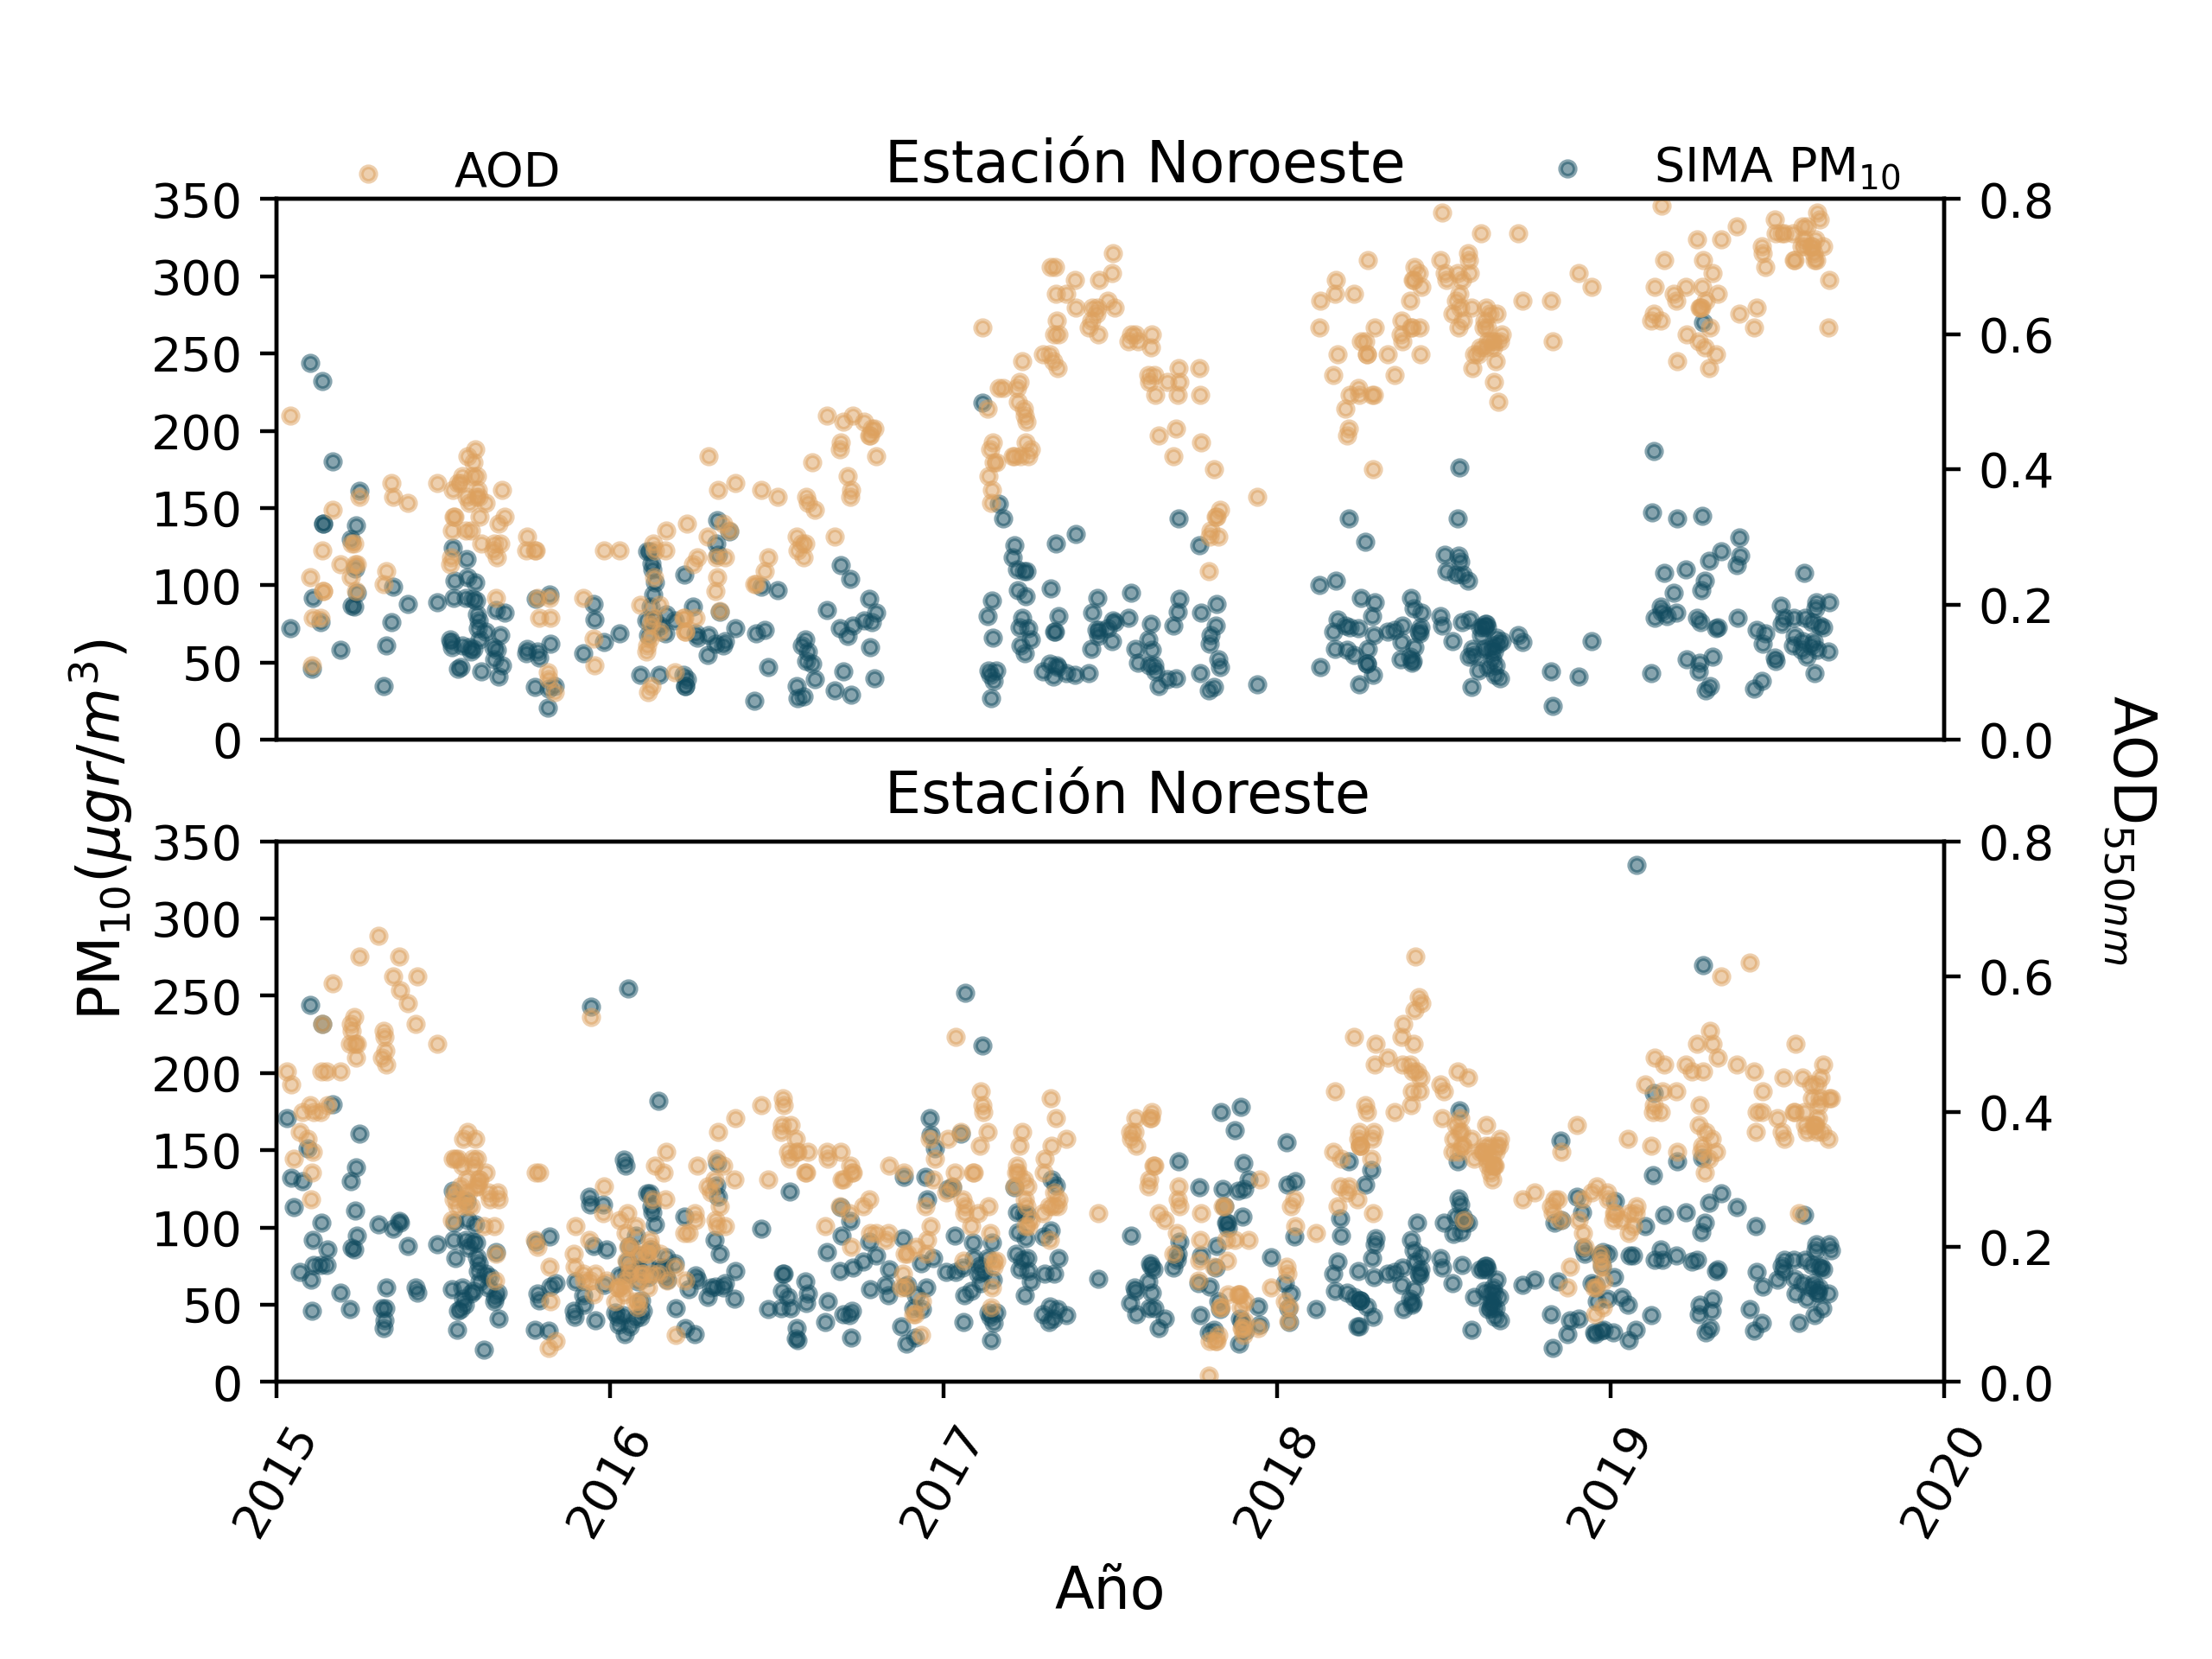
\includegraphics[height=8cm]{images/AODsandPM10.png}
        \caption{AOD\textsubscript{550nm} derivado del modelo SMARTS para el escenario Moderate al medio día solar en días de cielo despejado y PM\textsubscript{10} medido en las estaciones SIMA de la AMM durante el periodo 2015-2019.}
    \end{figure}
\end{minipage}
\begin{minipage}{0.45\linewidth}
    \begin{figure}[H]
        \centering
        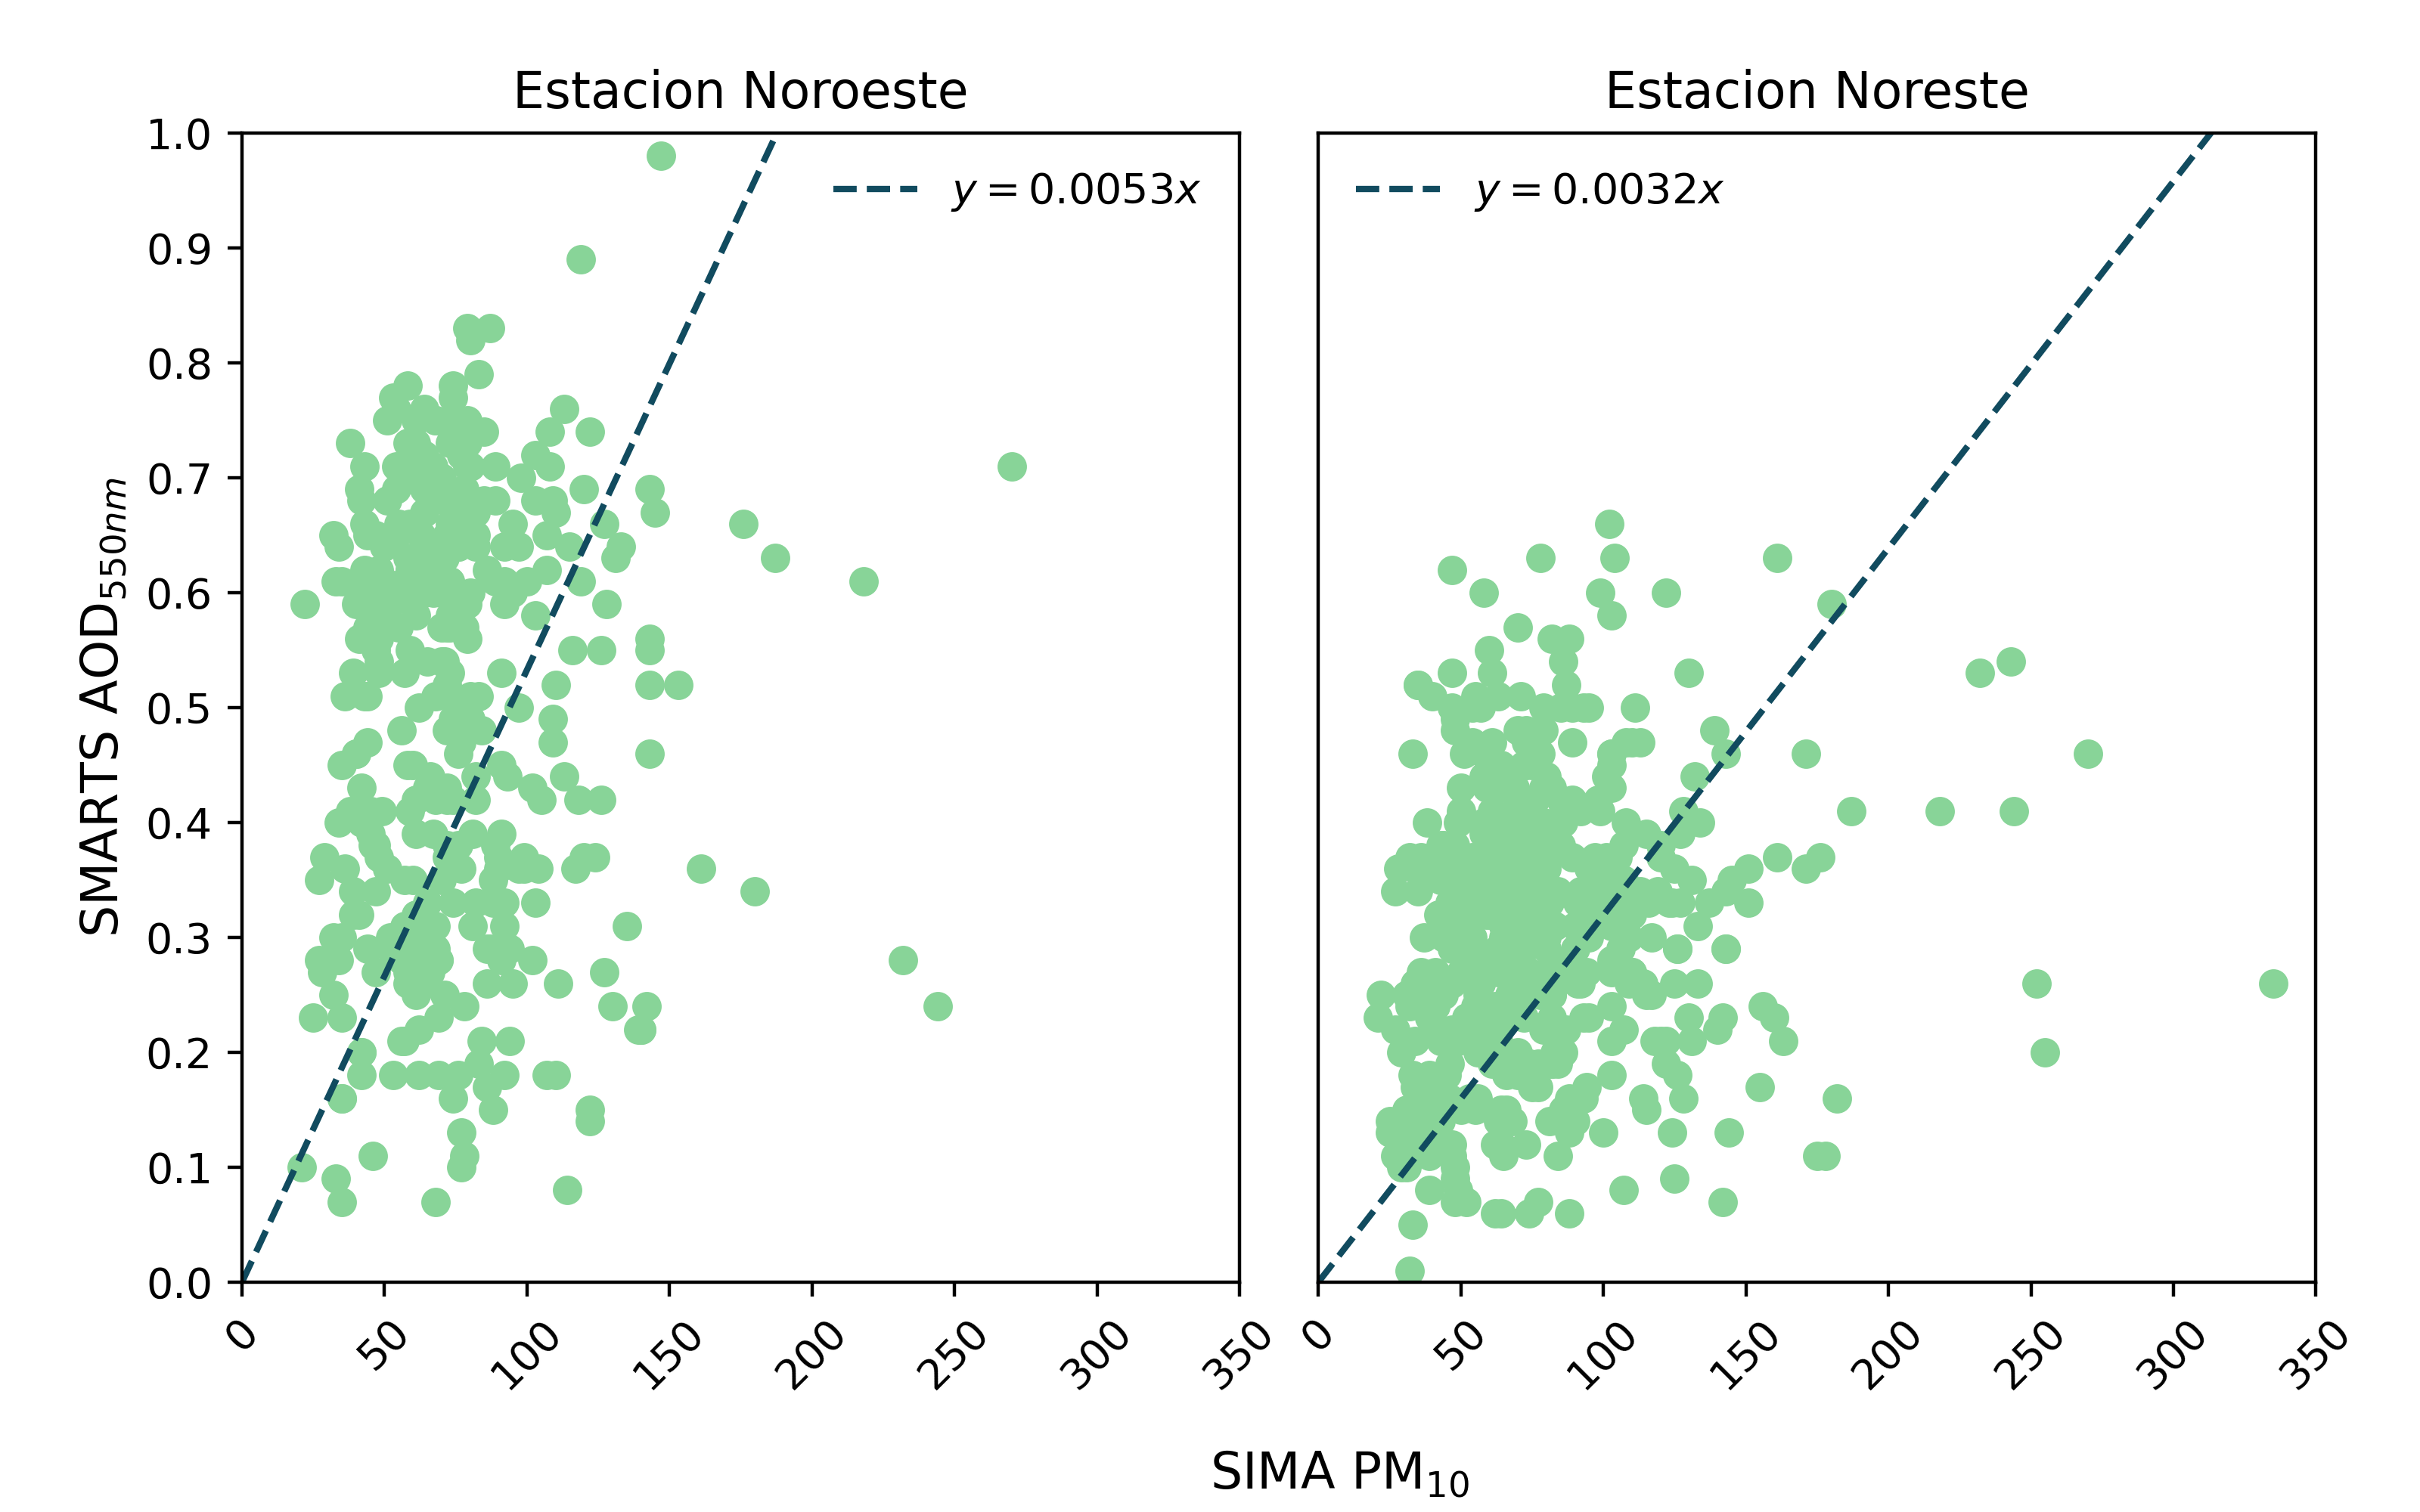
\includegraphics[height=7.5cm]{images/AODvsPM10.png}
        \caption{Correlación entre el AOD\textsubscript{550nm} obtenido con el modelo SMARTS con PM\textsubscript{10} medido en las estaciones SIMA del AMM para días de cielo despejado en el periodo 2015-2019.}
    \end{figure}
\end{minipage}
\end{center}
\begin{minipage}{0.60\linewidth}
\begin{center}
\begin{shaded}
\textbf{\textcolor{ver}{Conclusiones}}
\end{shaded}
\end{center}
\end{minipage}
\hspace{1cm}\vspace{0.5cm}
\begin{minipage}{0.35\linewidth}
\begin{center}
\begin{shaded}
\textbf{\textcolor{ver}{Referencias}}
\end{shaded}
\end{center}
\end{minipage}
\end{document}